% use the base acmart.cls
% use the sigplan proceeding template with the default 10 pt fonts
% nonacm option removes ACM related text in the submission. 
\documentclass[conference,10pt]{IEEEtran}
\usepackage{csvsimple}
\usepackage{subcaption}
\usepackage{cite}
\usepackage{amsmath,amsthm,amssymb,amsfonts,stmaryrd}
\usepackage{algorithmic}
\usepackage{graphicx}
\usepackage{xcolor}
\usepackage{booktabs}

\newcommand{\fixme}[1]{\textcolor{red}{#1}}
\newcommand{\todo}[1]{\textcolor{red}{TODO:\ #1}}
\newcommand{\fullname}{More Exact FPGA Technology Mapping with E-Graphs}
\newcommand{\shortname}{E-Pack}
\newcommand{\metric}{12\% fewer LUTs}
\newcommand{\fmetric}{45\%}
\newcommand{\nimproved}{45}
\newcommand{\nbenchmarks}{99}
\newcommand{\B}{\mathbb{Z}_{2}}
\newcommand{\Bk}{\mathbb{Z}_{2}^{k}}
\newcommand{\Bx}[1]{\mathbb{Z}_{2}^{#1}}

% enable page numbers
% \settopmatter{printfolios=true}


\begin{document}

\title{\fullname}
\author{\IEEEauthorblockN{Anonymous Authors}}
\maketitle

\begin{abstract}
    FPGA technology mapping is a well-studied problem and has been an area of
    interest in EDA tool design for decades. In most respects, the computational
    complexity of technology mapping is understood, and heuristic algorithms have
    been successfully employed to mitigate compile times while maintaining high QoR
    (quality of results). As transistor scaling comes to an end within the coming
    years, logic synthesis tools will become more of a bottleneck in the design of
    high performance accelerators. As a solution, we introduce E-Pack, an e-graph
    driven technology mapper that can better span the wide gap between SAT-based
    exact synthesis and heuristic cut enumeration techniques. We show that E-Pack
    can synthesize circuits with \metric{} on average---without ever
    increasing circuit depth. We also provide an empirical analysis of the runtime
    of E-Pack and show that it is still practical for large designs. Finally, we
    demonstrate that our compiler infrastructure is reusable, and future work can
    use our compiler for RTL equivalence checking or auditing the QoR of synthesis
    tools.
\end{abstract}

\section{Introduction}\label{sec:intro}
Given the complexity of modern electronic systems, a high degree of automation
is required to develop custom hardware within sensible timelines. At the
highest level, FPGA and ASIC design flows can be split into logical synthesis
and physical synthesis (optimize timing, placement and routing, etc..). This
division of work produces suboptimal designs, and neither are the individual
synthesis steps locally optimal on their own. However, logic minimization
problems in general are NP-Hard~\cite{logicmin,twolevellogic}, and modern EDA
flows bring compile times down to the human timescale while maintaining
acceptable QoR (quality of results).

With the end of Moore's Law scaling, chip area becomes a tighter constraint,
and logic synthesis is more of a bottleneck. Hence, future synthesis tools will
need to expand the design spaces they explore and find more optimal solutions.
Nonetheless, finding provably optimal circuits is computationally intractable.
In this paper, we will introduce how FPGA technology mapping can be augmented
with e-graph data structures to find \textit{more} exact solutions, without
significantly increasing compile times.

Technology mapping is the hand-off between logical synthesis and physical
synthesis. It converts the abstract Boolean logic into a network of gates that
belong to the target cell library. For FPGAs, the primary target cell is the
LUT (lookup table). Since every $k$-LUT can be re-programmed to satisfy any $k$
input boolean function, FPGA technology mapping has a unmistakably large
solution space. Whether the circuit is optimized for latency or area, most FPGA
tools approach technology mapping as a graph covering problem~\cite{flowmap,
    daomap, attmap, imap}. In the literature, a group of circuit nodes implemented
by a $k$-LUT is called a $k$-feasible cut of logic, and the generation of all
cuts is called cut enumeration. These structural mapping techniques
fundamentally rely on the topology of the input circuit. Hence, they are prone
to structural bias.

In contrast, functional mappers attempt to decompose Boolean functionality into
smaller sub-functions which can be realized by $k$-LUTs. Such mappers are a
more exact approach, and often use SAT solvers~\cite{satmap,satmap2} to drive
synthesis. However, exact synthesis tools cannot be scaled past tens of gates.
As a consequence, cut enumeration and functional mapping lie on two different
extremes. The former is faster but limited by the input structure, while the
latter is unbiased but fundamentally unscalable.

For this reason, we propose an e-graph driven technology mapper than can better
span the time-QoR spectrum. E-graphs are a data structure which use union-find
operations to compactly represent abstract equivalence relations. E-graphs are
useful as an optimizing compiler framework, because terms can be iteratively
rewritten in a nondestructive fashion. Instead of a optimization pass
architecture, e-graph driven compilers store all transformed terms in parallel
and defer selection of the best one. Our work seeks to evaluate the suitability
of e-graphs for logic synthesis, specifically technology mapping to FPGAs.

We introduce \shortname{}: a tool for repacking FPGA netlists into more compact
forms---without increasing circuit depth. Our results show many benchmarks, big
and small, which synthesize to significantly fewer LUTs over vendor EDA tools.
To that end, our work makes the following contributions:

\begin{itemize}
    \item We formulate an intermediate language and generating set of e-graph rewrite
          rules, as well as justify the types of circuit topologies that are reachable
          under composition.
    \item We evaluate our compiler against 96 benchmarks combined from three sources:
          EPFL~\cite{epflbench}, ISCAS'85~\cite{iscasbench}, and
          LGSynth'91~\cite{lgsynthbench}.
    \item \shortname{} is packaged as a Verilog-to-Verilog tool that can be dropped into existing RTL flows.
\end{itemize}

Before elaborating on our methodology and experimental setup, we first discuss
related ideas in technology mapping and e-graph driven compilers. Then, the
results section illustrates the typical reduction in LUT count our tool
achieves without increasing circuit depth. Lastly, we discuss the future work
of our compiler.
\begin{figure*}[tb]
    \begin{subfigure}{0.49\textwidth}
        \centering
        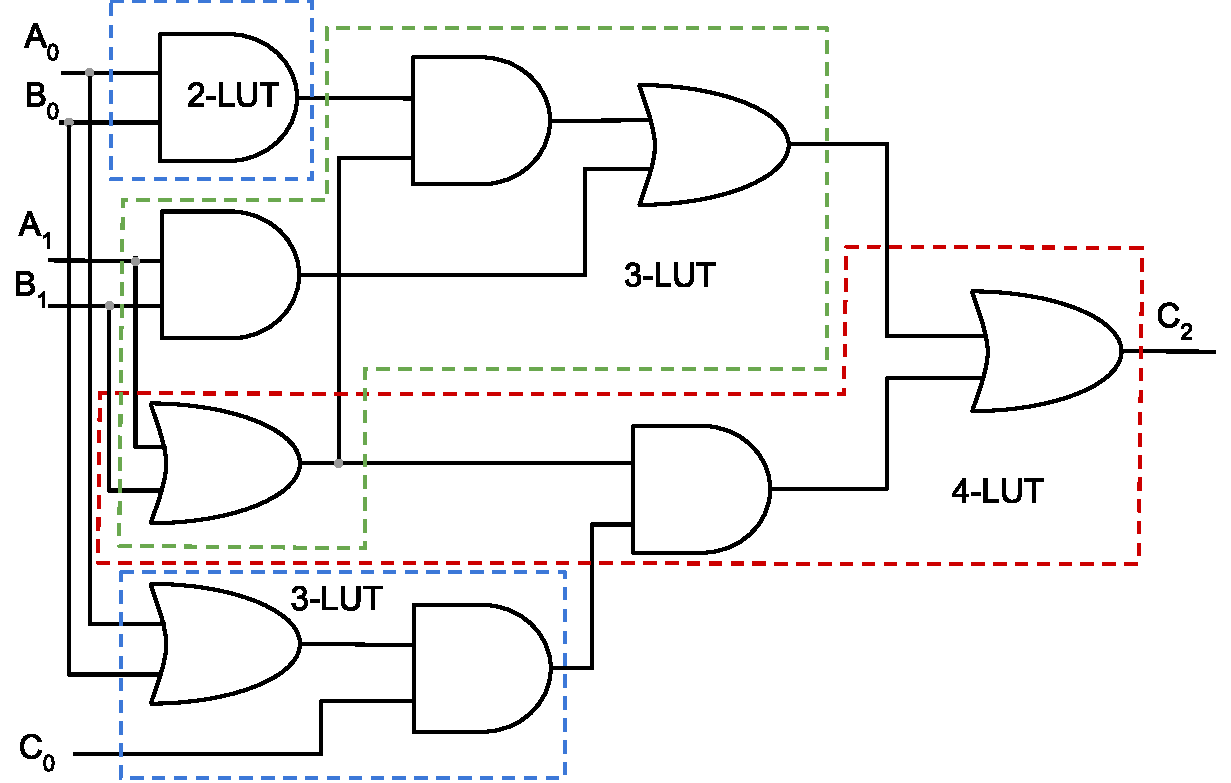
\includegraphics[width=0.92\textwidth]{img/cla_bad.pdf}
        \caption{An implementation that uses four LUTs contains redundancy.}\label{fig:eg:bad}
    \end{subfigure}
    \hfill
    \begin{subfigure}{0.49\textwidth}
        \centering
        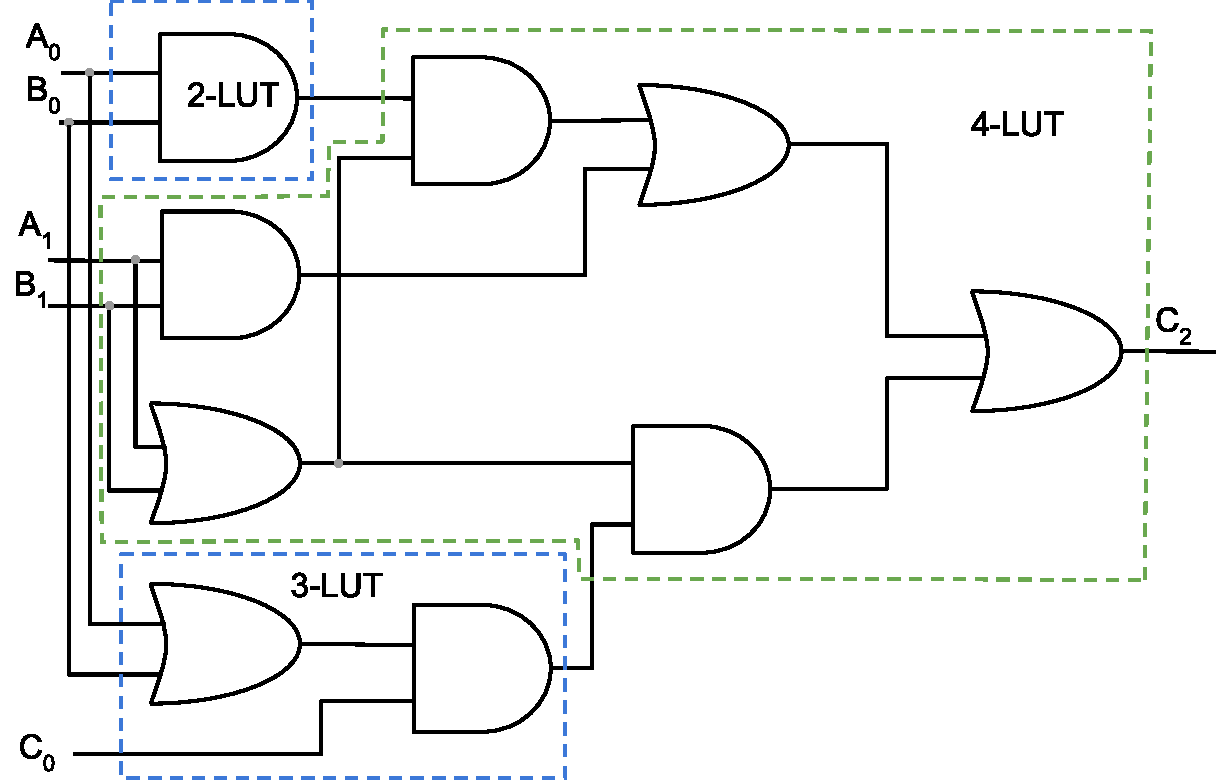
\includegraphics[width=0.92\textwidth]{img/cla_good.pdf}
        \caption{The sink cut of logic can expand its cover and reduce the LUT count by one.}\label{fig:eg:good}
    \end{subfigure}
    \caption{A 2-bit CLA (carry-lookahead) circuit demonstrates that non-monotone clustering can map suboptimally to a 4-LUT FPGA.}\label{fig:eg}
\end{figure*}

\section{Background}\label{sec:background}

\subsection{FPGA Technology Mapping}\label{sec:background:fpga}
FPGA technology mapping is the compilation step that converts abstract RTL
logic into a netlist of lookup tables~\cite{flowmap, daomap, attmap, imap,
    wiremap}. Due to the computational complexity of optimal LUT packing, most
implementations avoid restructuring the input logic and are essentially graph
covering algorithms. Given a $k$-LUT FPGA architecture, most mappers start by
enumerating the feasible cuts of logic for each node in the circuit. Then,
logic cuts are selected to be used in the circuit covering, which ultimately
becomes the netlist. Where competing implementations vary, however, is the set
of heuristics used to extract the best cuts of logic. The heuristic nature of
these algorithms means that results can be inconsistent across implementations,
and the discrepancies are difficult to explain.

As an example, Fig.~\ref{fig:eg} shows two different results of mapping
carry-lookahead logic to a 4-LUT FPGA architecture. In Fig.~\ref{fig:eg:bad},
the circuit is implemented with four total LUTs. Since the sink LUT is already
utilizing all four inputs, the ability to combine it with another 4-LUT is
non-obvious. Fig.~\ref{fig:eg:good} shows how the circuit depth and cell count
can both be reduced by merging the two 4-LUTs, because they both share the
inputs $A_1$ and $B_1$. This feature in the circuit topology is referred to in
the literature as \textit{non-monotone clustering} of logic~\cite{flowmap}. In
other words, a $k$-feasible cut of logic may contain within itself cuts of
logic that are the same size or even larger. That is, traversing subcuts does
not decrease the cut size monotonically. Hence, technology mapping must
scrutinize this type of circuit topology in order to avoid suboptimal LUT count
and depth, adding to tool runtime. It is important to note that this problem
occurs equally on 6-LUT FPGAs.

\textit{Not} depicted in Fig.~\ref{fig:eg} is the bias the graph
covering has to the structure of the input logic. Depending on how the input
RTL is written, the optimal solution may not be reachable with a cut
enumeration algorithm. First, notice that both the AND and OR operations in the
circuit are commutative and associative. A poor grouping of terms can limit the
efficacy of the technology mapper. In this specific case, it is important that
$C_0$ is grouped with $A_0 + B_0$ and \textit{not} $A_1 + B_1$. To summarize,
technology mapping must overcome both the difficulty of cut selection
and bias toward the structure of the input circuit.

\subsection{Equality Graphs}\label{sec:background:egraph}
Equality graphs, most commonly referred to as \textit{e-graphs}, are an
automated reasoning tool built around a union-find data
structure~\cite{eggpaper, eqsat}. E-graphs are particularly strong at
equational reasoning. For example, e-graphs can be used to rewrite mathematical
expressions~\cite{egraphmath} or for automated reasoning about functional
programs~\cite{cclemma}. Briefly put, e-graphs can drive logic synthesis by
exploring other circuit topologies. Initially, each circuit node starts alone
in its equivalence class. Then, a set of rewrite rules is used to grow the
e-graph with alternative representations. When rewrite rules no longer
introduce new information into the graph, we say we have reached
\textit{equality saturation}.

Equality saturation is useful for optimizing compilers, because it defers
greedy program transformations. Extracting solutions from saturated e-graphs
can result in more optimal---sometimes provably optimal---programs. In
contrast, traditional compilers use a pass pipeline architecture which suffers
from a \textit{phase-ordering problem}. In other words, there is never an
ordering of transformation passes that is optimal for all input programs. This
is a deep-rooted issue in compiler design, but the problem is particularly
consequential for hardware design. The exploratory nature of e-graphs are
useful for combinatorial problems like LUT-based technology mapping.

\section{Related Work}\label{sec:relatedwork}
\subsection{LUT Packing}\label{sec:relatedwork:fpga}
\zz{we need to first introduce the concept of LUT packing, if it's not described earlier}
Broadly speaking, FPGA LUT packing can be divided into architecture-specific
and architecture-nonspecific optimizations. \zz{the more common term is architecture-agnostic or -independent} Architecture-specific LUT packing
can reduce routing congestion by more efficiently using intra-CLB routing
resources. Examples include mapping dual-output functions to fractured
LUTs~\cite{fraclut} or using dedicated multiplexers to implement functions with
more than 6 inputs~\cite{ug574}. The rough optimization goal of LUT packing is
to reduce the number of flip-flops driven across CLB boundaries~\cite{ffpack}.

In contrast, architecture-nonspecific LUT packing is \fixme{broader} as it
attempts to mitigate the structural bias of the technology mapper in general.
\zz{broader in what sense?} As an example, AGDMap~\cite{adaptdecomp} decomposes
simple logic gates with large fanin to enable the exploration of better graph
coverings. However, structural bias can take on many forms. Finding
advantageous decompositions of logic in general requires more elaborate
algorithms~\cite{dsd} that may not be practical for large designs. \zz{AGDMap
    is a tech mapping paper and it does not use the term LUT packing}
FlowMap~\cite{flowmap} cites non-monotone clustering of logic as the
fundamental difficulty that causes bias in LUT-based technology mapping. In
other words, this is the observation that a $k$-feasible cut of logic may
contain subcuts that are \textit{not} $k$-feasible. Overcoming \fixme{bouts}
\zz{is it a common term?} of non-monotone clustering requires a more elaborate
cut-selection algorithm, and our work lays the foundation for a formal,
reasoning-based approach to the problem.

\subsection{E-Graph Superoptimization}\label{sec:relatedwork:egraph}
In recent years, e-graphs and equality saturation have enjoyed renewed
popularity within the compilers field. Several recent works use e-graph driven
superoptimization to improve upon existing EDA tool flows. SEER~\cite{seer}
uses e-graphs to optimize and parallelize the control flow of high-level
synthesis (HLS) programs. IMpress~\cite{impress} also uses e-graphs at the HLS
level, optimizing the datapath of large bit-width multipliers. At a lower
level, ROVER~\cite{rover,roverbl,egraphconstraints} rewrites arithmetic data
paths at the word and bit levels. ROVER straddles the RTL and physical level of
abstraction, making it more general purpose than IMpress. In any case, the work
which is most similar in its goals to ours is E-Syn~\cite{esynth}. E-Syn uses
Boolean algebra to rewrite a circuit with known properties like De Morgan's
laws and the consensus theorem. Ultimately, E-Syn performs its optimizations
during technology-independent synthesis steps, whereas \shortname{} applies as
a post-processing step \textit{after} technology mapping. Furthermore,
\shortname{}'s rewriting system models the netlist in terms of total functions,
rather than as expressions over a Boolean algebra.
\section{E-Graph Construction}\label{sec:rewrites}
As an overview, an e-graph is built by accumulating new equivalence relations
through the iterative rewriting of terms. Rewrite rules define the equivalence
relations in full generality by designating a search pattern of terms to
rewrite. This prompts the creation of a grammar that can represent the
structure of electronic circuits and lends itself well to pattern matching. As
an example, one can write De Morgan's laws as rewrite rule:

\begin{lstlisting}
(NOT (AND x y)) => (OR (NOT x) (NOT y))
\end{lstlisting}

The left-hand side is the search pattern, and the right-hand side describes how
to apply the rewrite to the pattern. Rewrites must be merged back into the
union-find data structure, so this is an iterative process. In the following
subsections, we will define our netlist representation, \texttt{LutLang}, and
the accompanying equivalence relations. Formalizing the meaning of FPGA
netlists is critical to both ensuring correctness and finding deeper insight
into the structure of our rewrite rules under composition.

\subsection{\texttt{LutLang} Representation}\label{sec:rewrites:lutlang}

Input Verilog netlists are converted to our internal format, called
\texttt{LutLang}, which is compatible with e-graph structures. When printed to
text, \texttt{LutLang} takes on a Lisp-like syntax and our rewrite rules are
written in such style. As an example, a 2-LUT cascaded into a 3-LUT is written
as follows:

\begin{lstlisting}
(LUT G x2 x3 (LUT F x0 x1))
\end{lstlisting}

\texttt{G} and \texttt{F} are the truth-tables of the LUTs.
We also call them the \textit{program} or \textit{function} interchangeably.
Since $k \leq 6$, truth tables are stored as 64-bit integers, but we analyze them as total functions $F: \Bk \rightarrow \B$.
To clarify notation, $\mathbb{Z}_2 = \mathbb{Z}/2\mathbb{Z} = \mathbb{B} = \{0,1\}$.
To that end, the denotational semantics $\llbracket \cdot \rrbracket : \texttt{LutLang} \rightarrow \mathbb{Z}_2$ of a LUT is simply applying its Boolean inputs to the function:

\begin{equation}
    \llbracket \texttt{(LUT F x0 x1)} \rrbracket = F(\llbracket \texttt{x0} \rrbracket, \llbracket \texttt{x1} \rrbracket)
\end{equation}

\begin{figure}
    \centering
    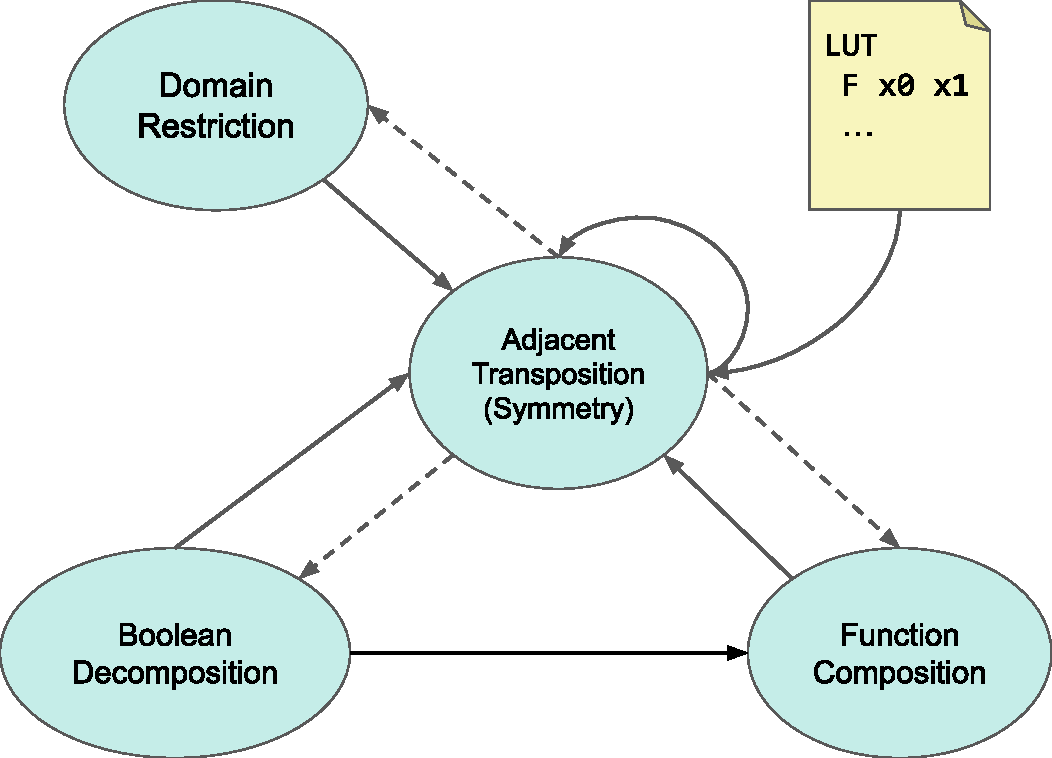
\includegraphics[width=0.47\textwidth]{img/rewrites.pdf}
    \caption{Transition diagram of rewrite rules. A solid arrow means that the application of the source rule always becomes an instance of the target rule.}\label{fig:rewrites}
\end{figure}

\subsection{Simplifying Degenerate LUTs}\label{sec:rewrites:degen}

\textbf{Definition:} A LUT's configuration $F : \Bk \rightarrow \B$ is \textit{degenerate} if there exists a Shannon expansion $F = x_i \cdot F_{x_i} + \overline{x_i} \cdot F_{\overline{x}_i}$
such that $F_{x_i} = F_{\overline{x}_i}$ for some input position $i \in \{ 0, \ldots, k -1\}$. In other words, $F = F_{x_i} = F_{\overline{x}_i}$.

The output of a degenerate LUT is not dependent on one of its inputs. Hence, it
can be rewritten into a LUT which uses fewer inputs. This rule is applied by
computing the Shannon expansions of LUTs and checking for equivalence. As an
example, the rule takes on the following form in pseudocode for $k=3$:

\begin{lstlisting}
(LUT F x0 x1 x2) => (LUT F' x0 x1)
    if F(x0, x1, false) == F(x0, x1, true)
    where F'(x0, x1) := F(x0, x1, true)
\end{lstlisting}

On the left of \texttt{=>} is the \textit{search pattern}. The right-hand side
of the rule is the \textit{application}. One rule is instantiated for each LUT
size $k =1$ through 6. One should notice that LUTs which are constant functions
are also handled by this rule. Since this rule is computationally expensive, it
is applied greedily as a pre-processing step before the e-graph is built. None
of the other rewrite rules create degenerate LUTs, so this has no impact on
results.

\subsection{Partial Application}\label{sec:rewrites:application}
A LUT with a constant input can be partially evaluated to a LUT with one less
input. This rule is similar to the last. It computes the Shannon expansion
along the constant variable and chooses the cofactor that matches the state of
the constant input. One could show that applying this rule greedily in
combination with the previous one is equivalent to constant propagation. As an
example, the pseudocode for $k=3$ is written as follows:

\begin{lstlisting}
(LUT F x0 x1 false) => (LUT F' x0 x1)
    where F'(x0, x1) := F(x0, x1, false)
\end{lstlisting}

\subsection{LUT Symmetries}\label{sec:rewrites:symmetry}

The semantics of LUTs should not depend on the order of their inputs. If two
LUTs have permuted inputs but are otherwise functionally identical, they should
belong to the same e-class in the graph. That is, \mbox{\texttt{(LUT F .. xi ..
        xj ..)}} is semantically equivalent to \mbox{\texttt{(LUT G .. xj .. xi ..)}}
if and only if $G = F \odot \sigma^{-1}$, where $\sigma \in S_k$ is the
permutation applied to the inputs.

\begin{proof}
    $\odot$ is a right-action defined for the sake of permuting the inputs to a function before they are applied:
    \begin{equation*} \odot : \big (\Bk \rightarrow \mathbb{Z}_2 \big ) \times S_k \rightarrow \big (\Bk \rightarrow \mathbb{Z}_2 \big ) \end{equation*}
    \begin{equation*} F \odot \sigma : (x_0, x_1, \ldots, x_{k-1}) \mapsto F(x_{\sigma(0)}, x_{\sigma(1)}, \ldots, x_{\sigma(k-1)}) \end{equation*}

    It is trivial to prove that this right-action is associative:
    \begin{align*}
        (F \odot \sigma_1) \odot \sigma_2 & = F(x_{\sigma_2(\sigma_1(0))}, x_{\sigma_2(\sigma_1(1))}, \ldots, x_{\sigma_2(\sigma_1(k-1))}) \\
        (F \odot \sigma_1) \odot \sigma_2 & = F \odot (\sigma_2 \circ \sigma_1)
    \end{align*}
    With this property, the rest follows directly:
    \begin{equation}
        F = G \odot
        \sigma \iff F \odot \sigma^{-1} = (G \odot \sigma) \odot \sigma^{-1} = G
    \end{equation}
\end{proof}

Therefore, we can conclude that $k$-LUTs have as much symmetry as can be
generated by the group $S_k$. The insight from this formal approach has two
main consequences. First, it precisely reveals how many e-graph rewrite rules
are needed to generate all the symmetries of a LUT. For any $k$-LUT with
program $F$, we need exactly as many rules as it takes to generate $F \odot
    S_k$. It is a well-known fact in algebra that the $k-1$ adjacent transpositions
generate $S_k$~\cite{sgroup}. Therefore, we can insert an e-graph rewrite rule
for each adjacent transposition. In total, there are $\sum_{k=2}^{6} (k-1) =
    15$ rules to encapsulate symmetry for every LUT size. The second consequence is
that every other rewrite rule can now be defined for one input position,
without loss of generality. This reduces the total number of rewrite rules,
making it easier to rationalize about the rule system and which types of
optimizations are reachable.

\subsection{Function Composition}\label{sec:rewrites:composition}

Cascaded LUTs can be packed into a single LUT, as long as the size of the cut
of logic has at most 6 leaf nodes. This is the crucial observation to LUT
packing. For instance, a circuit that implements $F(x_0, G(x_1, x_2))$ with two
2-LUTs can be rewritten as a 3-LUT that implements some $H(x_0, x_1, x_2)$. In
pseudocode, this would take on the following form:

\begin{lstlisting}
(LUT F x0 (LUT G x1 x2)) => (LUT H x0 x1 x2)
    where H(x0, x1, x2) := F(x0, G(x1, x2))
\end{lstlisting}

The search patterns \texttt{x0}, \texttt{x1} and \texttt{x1} can match any
node. They are not necessarily principal inputs, and hence can be outputs from
other LUTs. As a consequence, this rule can be chained together many times in
different orders to pack a sub-circuit into a single LUT. As a consequence of
the previous rule, we can write compositions for one specific input position,
without loss of generality. Therefore, we only need to sweep over the size of
the two LUTs in the search pattern. In total, there are $6*6 = 36$ LUT packing
rules. When the cut of logic is larger than 6 leaves, the rule exits gracefully
and do not interfere with reaching equality saturation.

\subsection{LUTs with Domain Restrictions}\label{sec:rewrites:restrict}

\zz{we could use an example here. Fig 1 is currently only used in the background. Ideally we want to refer to it (or a different example) again when we discuss some of the rewrite rules}

\textbf{Definition:} A lookup table \texttt{(LUT F x0 x1 \ldots)} is \textit{restricted} if $\llbracket \texttt{xi} \rrbracket = \llbracket \texttt{xj} \rrbracket$ for some $ i, j \in \{0, \ldots, k-1\}, \; i \neq j$.
In other words, the domain of the LUT is restricted.

The main advantage of using e-graphs is the compact way in which it represents
notions of equality. Whenever a new equivalence is found between two of the
inputs to a $k$-LUT, it can be rewritten with a $(k-1)$-LUT. We simply need to
define and compute $\texttt{restrict(F, i, j)}$ which maps $F : \Bx{k}
    \rightarrow \B$ to the domain-restricted $F \vert_{x_i = x_j} : \Bx{k-1}
    \rightarrow \B$. In pseudocode, the rewrite rule can be rewritten as follows:

\begin{lstlisting}
(LUT F x0 x1 x1) => (LUT F' x0 x1)
    where F' := restrict(F, 1, 2)
\end{lstlisting}

Since rewrite search patterns already match `modulo' e-class, this rule is
automatically triggered when e-classes are merged. Since LUT symmetry is
represented in the graph, only one rule is needed for each LUT size $k=2$
through 6.

\begin{figure*}[tb]
    \begin{subfigure}{0.31\textwidth}
        \centering
        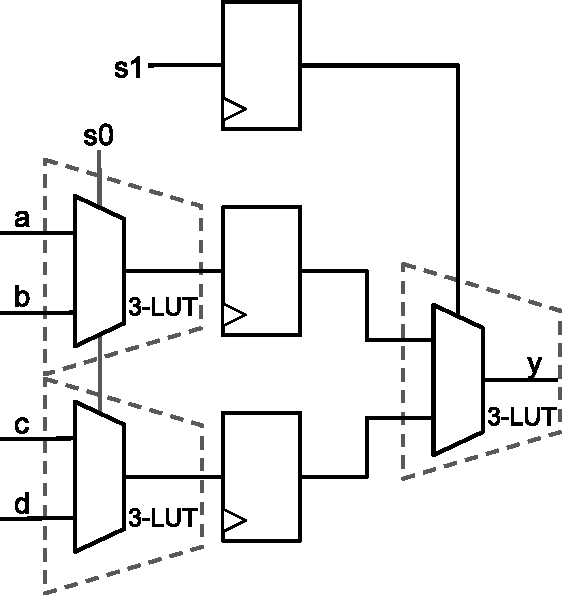
\includegraphics[width=0.88\textwidth]{img/mux_4_1.pdf}
        \caption{Three 3-LUT, three FF topology.}\label{fig:retiming:a}
    \end{subfigure}
    \begin{subfigure}{0.38\textwidth}
        \centering
        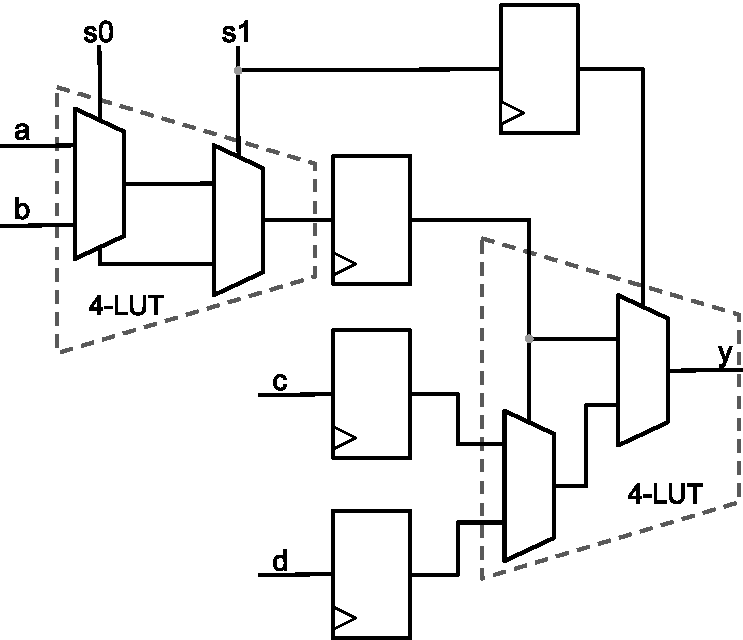
\includegraphics[width=0.9\textwidth]{img/mux_4_1_retime_dsd.pdf}
        \caption{Two 4-LUT, four FF topology.}\label{fig:retiming:b}
    \end{subfigure}
    \begin{subfigure}{0.30\textwidth}
        \centering
        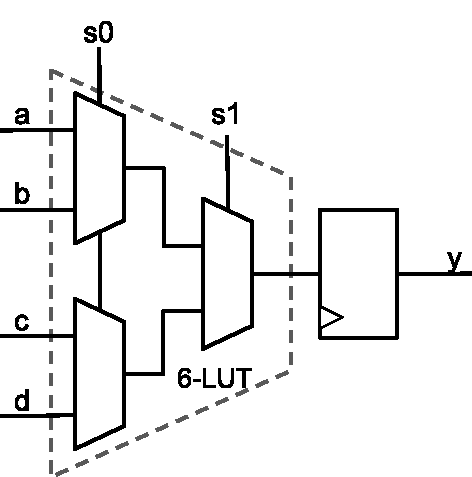
\includegraphics[width=0.84\textwidth]{img/mux_4_1_retime.pdf}
        \caption{One 6-LUT, one FF topology.}\label{fig:retiming:c}
    \end{subfigure}
    \caption{Three varying topologies for 4:1 MUX with pipeline register.}\label{fig:retiming}
\end{figure*}

\subsection{Functional Decomposition}\label{sec:rewrites:decomp}

Decomposing boolean functions and logic minimization in general is
NP-complete~\cite{logicmin}. Correspondingly, decomposing LUTs explodes the
size and build time of the e-graph. However, we can still define rewrites that
look for fully disjoint decompositions in one or more variables. This rule has
no structural element to search for, so it runs every time an e-class is
updated. Our implementation computes the Shannon expansion of a $k$-LUT's
function $F$ and checks that both cofactors are cognates in a loose sense. For
instance, given $k=3$ then it is true that for $G, H \in \B^2 \rightarrow \B$
that:

\begin{gather}
    F(x_0, x_1, x_2) = G(x_0, H(x_1, x_2)) \nonumber \\
    \Big\Updownarrow                       \nonumber \\
    F(x_0, x_1, x_2) = x_0 \cdot G_{x_0} (H(x_1, x_2)) +  \overline{x_0} \cdot G_{\overline{x}_0} (H(x_1, x_2))
\end{gather}

In practice, our implementation checks if either of the cofactors $G_{x_0}$ or
$G_{\overline{x}_0}$ are constant functions or if the cofactors are equivalent
up to complementation.

\subsection{Register Retiming}\label{sec:rewrites:retiming}

Register retiming is a purely structural rule, meaning it can be implemented
with a simple search and apply pattern. An example for $k=1$ would be written
as follows:

\begin{lstlisting}
(LUT F (REG x0)) <=> (REG (LUT F x0))
\end{lstlisting}

Unlike the other rules, this rule is searched for in both directions.
Figure~\ref{fig:retiming} illustrates an example of how register retiming can
compose with LUT rewrite rules to reduce LUT count and register count
simultaneously. In this case, the 3-LUTs implementing 2:1 multiplexers are
pushed across register boundaries. Since this logic happens to have a 6-LUT
packing and a two 4-LUT packing, we can explore a circuit topology that reduces
cell count (Fig.~\ref{fig:retiming:c}) or adjusts the delay paths
(Fig.~\ref{fig:retiming:b}). To best utilize register retiming, the e-graph
extraction technique must have some sense of timing information. Our e-graph
extractor is explained in the next section, but it should be noted that in our
experiments the area of LUTs and registers are weighted equally.
\begin{figure}
    \begin{subfigure}{0.47\textwidth}
        \centering
        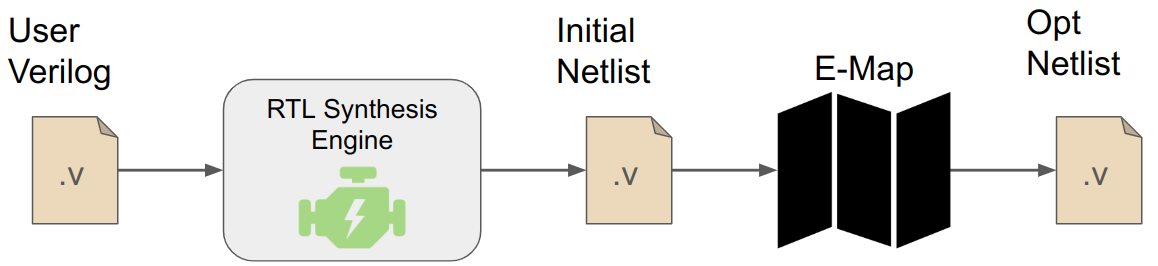
\includegraphics[width=\textwidth]{img/flow.png}
        \caption{The tool flow integrating E-Pack with existing RTL engines.}\label{fig:flow:rtl}
    \end{subfigure}
    \hfill\vspace{4mm}
    \begin{subfigure}{0.47\textwidth}
        \centering
        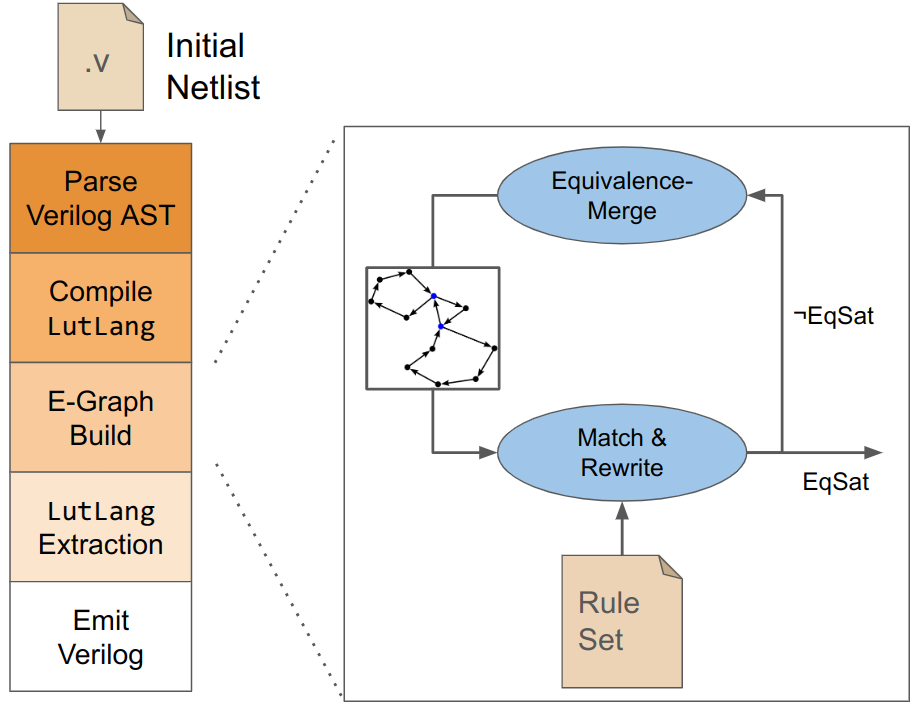
\includegraphics[width=\textwidth]{img/egraph.png}
        \caption{The compilation steps internal to \shortname{} Verilog tool.}\label{fig:flow:egraph}
    \end{subfigure}
    \caption{Diagrams of the top-level integration of E-Pack into existing tool flows and internal e-graph driven compiler architecture.}\label{fig:flow}
\end{figure}

\section{Tool Flow}\label{sec:flow}

While constructing the e-graph is the crux of \shortname{}, there are several
other important components to consider in the full design flow. In order to
test our hypothesis, \shortname{} must be compatible with existing synthesis
flows, and the rewritten circuits must be verified.

\subsection{Extraction}\label{sec:flow:extraction}
Regardless of whether equality saturation is achieved or not, the quality of
the output circuit still largely depends on the extraction technique used. In
short, \textit{extraction} is the process of selecting the ``best'' circuit
from the e-graph. Given that a saturated e-graph can contain hundreds of
thousands of e-nodes across tens of thousands of e-classes, a greedy extraction
algorithm is the most pragmatic. The greedy extractor iterates over the
e-classes, updating the cost of the cheapest e-node until the database of costs
no longer change. Whenever possible, our compiler uses the builtin
functionality of the egg e-graph Rust library~\cite{docsEgg}. However, e-graph
extraction itself is an ongoing research area~\cite{smoothe,
    sparsextract,esynth}, and future work should experiment with different
extraction algorithms. In any case, the greedy cost of a LUT is always one plus
the sum of the costs of its children nodes. Further subtle interactions between
extraction and the rewrite rule set are further explained in
Section~\ref{sec:results:margin}.

\subsection{Verilog Support}\label{sec:flow:verilog}
In order for our compiler to be compatible with as many existing design flows
as possible, some level of Verilog support is necessary. Our compiler supports
a subset of Verilog 2001~\cite{verilog}, as required to represent structural
netlists. This includes support for non-ANSI C style module declarations,
wires, and module instantiations with named port connections. With Verilog
support, we are able to test \shortname{} with tool flows that use
Yosys~\cite{yosys} or Vivado~\cite{vivado}. On the backend, our compiler also
emits an updated Verilog netlist.

\subsection{Verification}\label{sec:flow:verification}
While formal verification is not the primary focus of this work, using e-graphs
as a formal reasoning tool helps to build trust in our synthesis results. In
fact, e-graphs were originally designed for automated theorem
proving~\cite{eggpaper}. Thus, constructing proofs that demonstrate equivalence
between the original and optimized netlist is a builtin feature of
\shortname{}. This technique is relatively slow, so we also use two other
independent sources of verification. For combinational netlists, our middle end
can do exhaustive functional testing. Lastly, we use Yosys~\cite{yosys} for its
SAT-driven equivalence checking capabilities. All in all, the mixed usage of
these verification techniques build confidence in the robustness of our
technology mapper built around e-graphs.
\section{Results}\label{sec:results}
Our experiments were carried out on a Red Hat 8 server hosting a Intel Xeon
Gold 6242 CPU. Since \shortname{} is written in Rust, it mostly uses the
built-in functionality of the egg library. The egg e-graph runner was ran in a
time-limited configuration, meaning there was no limit in the size of the
e-graph. The specific time limit for e-graph construction was 10 minutes. In
most cases, the test circuit saturated the e-graph well before this time
limit---around 30 seconds. \shortname{} was evaluated against circuits from
three benchmark suites: EPFL~\cite{epflbench}, ISCAS'85~\cite{iscasbench}, and
LGSynth'91~\cite{lgsynthbench}. However, we also included an ALU and pipelined
multiplication module to test how our compiler behaves with increasing levels
of bit-parallelism and register pipelining. Finally, we measure how our mapping
optimizations influence CLB usage and timing closure.

\subsection{Benchmarking}\label{sec:results:benchmark}
\begin{table}
    \centering
    \csvautobooktabular{data/results.csv}
    \caption{Results of \nimproved{} improved benchmarks from ISCAS'85~\cite{iscasbench}, LGSynth'91~\cite{lgsynthbench}, and EPFL~\cite{epflbench}}\label{tab:results}
\end{table}

\begin{figure}
    \begin{subfigure}{0.47\textwidth}
        \centering
        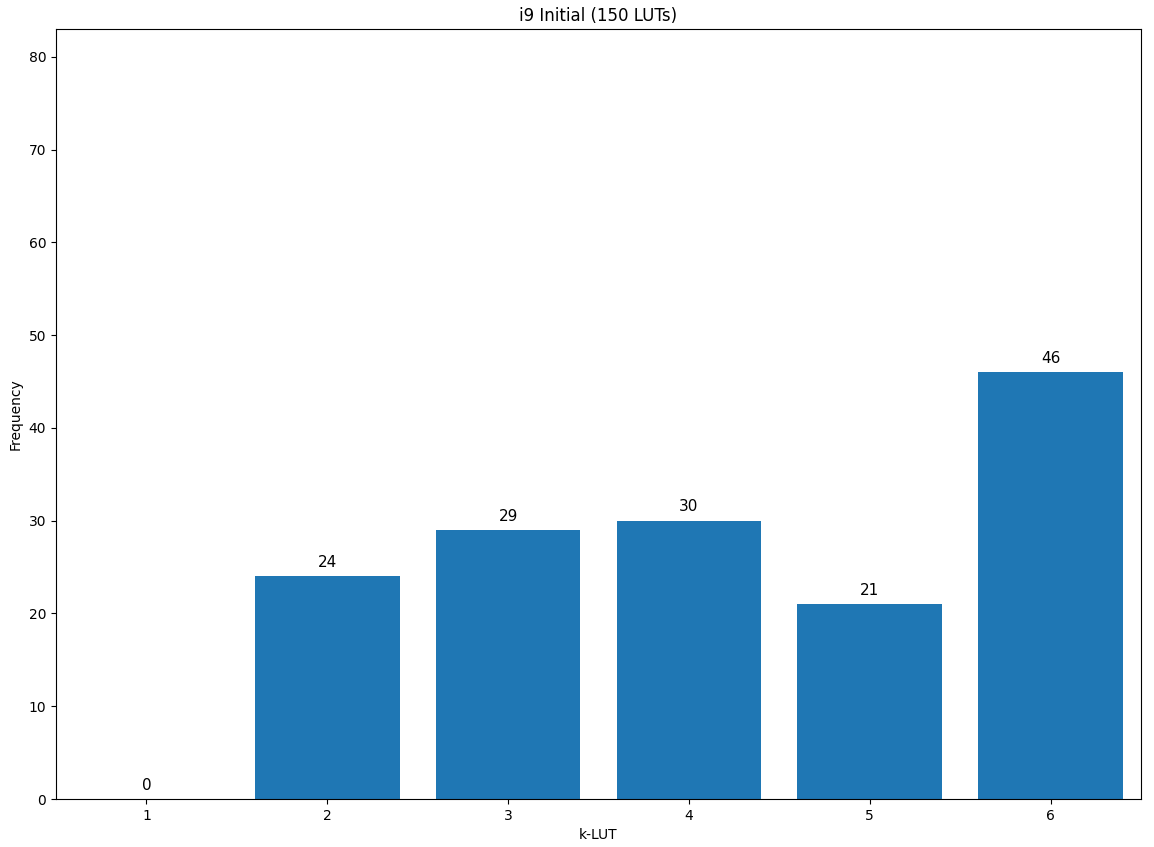
\includegraphics[width=\textwidth]{img/y33.png}
        \caption{Distribution of 150 LUTs after synthesis of `i9' with Yosys 0.33}\label{fig:histogram:y33}
    \end{subfigure}
    \hfill\vspace{4mm}
    \begin{subfigure}{0.47\textwidth}
        \centering
        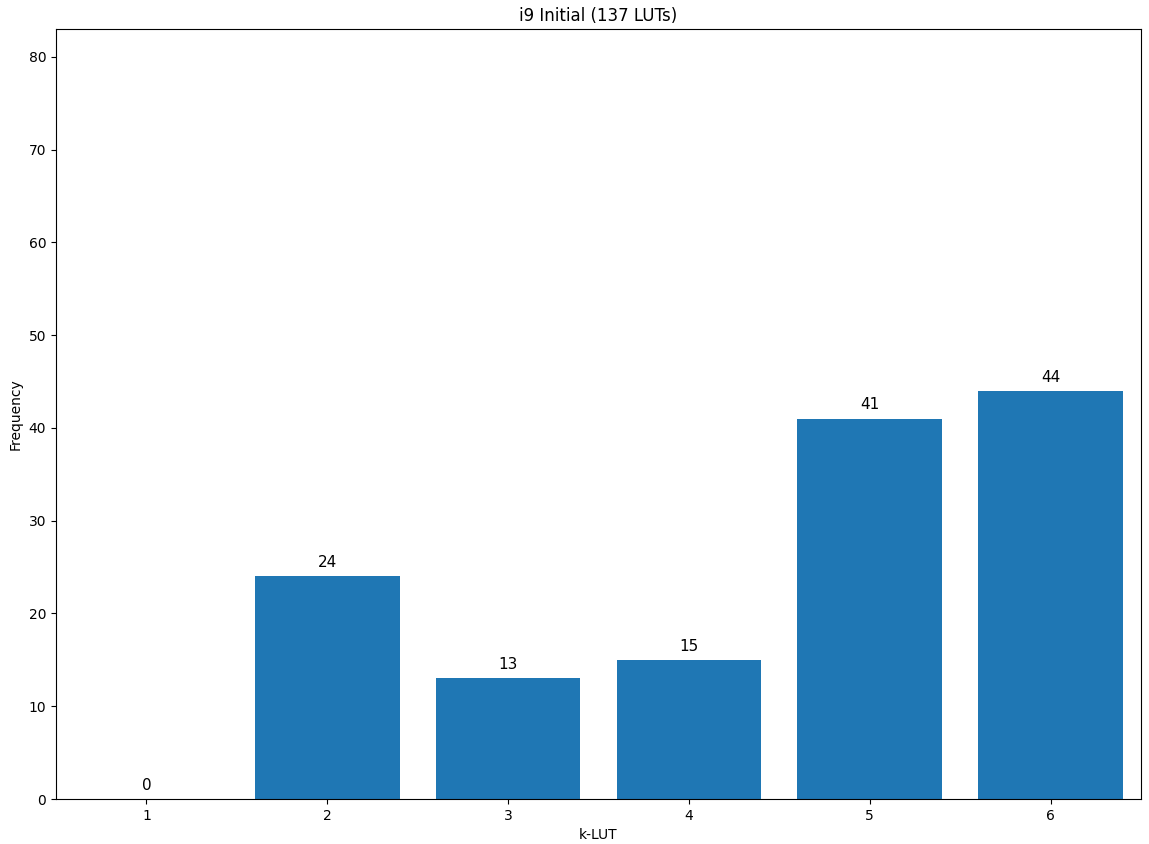
\includegraphics[width=\textwidth]{img/y44.png}
        \caption{Distribution of 137 LUTs after synthesis of `i9' with Yosys 0.44}\label{fig:histogram:y44}
    \end{subfigure}
    \hfill\vspace{4mm}
    \begin{subfigure}{0.47\textwidth}
        \centering
        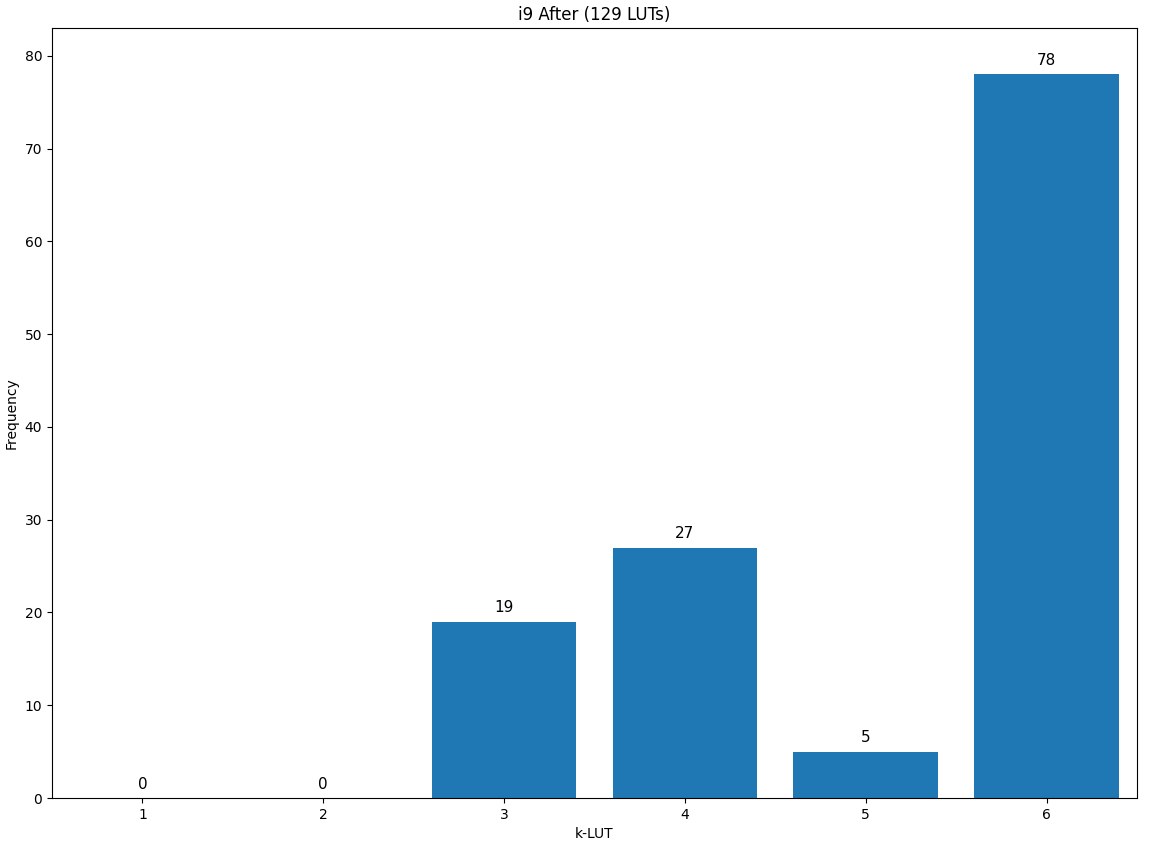
\includegraphics[width=\textwidth]{img/epack.png}
        \caption{Distribution of 129 LUTs after synthesis of `i9' with Yosys 0.3 + \shortname{}}\label{fig:histogram:epack}
    \end{subfigure}
    \caption{Comparison of two initial structures, (a) and (b), and E-Packed structure (c) \todo{regenerate these figs}}\label{fig:histogram}
\end{figure}

We used an compilation of \nbenchmarks{} combinational benchmarks from three
academic sources to test LUT packing ability. Among the combinational
benchmarks we tested, \shortname{} was able to reduce the LUT count \fmetric{}
of the time. On average, \shortname{} packed the netlists to \metric{}. The
results in Table~\ref{tab:results} list all the reduced LUT counts, sorted by
approximate design size. AMD/Xilinx Vivado 2024~\cite{vivado} was used as the
baseline synthesis tool. For the E-Pack flow, Yosys~\cite{yosys} is used to
generate the initial mapped circuit. At a glance, circuits like `int2float,'
`c6288,` `adder,' and `square' have the most to gain from \shortname{}. These
circuits are all arithmetic in nature, and this is a common occurrence
throughout the rest of the results.

One result that is \textit{not} demonstrated by the table is the apparent
importance of the initial structure inputted to E-Pack. We have not eliminated
all sources of structural bias, and hence our superoptimization tool still
occasionally gets stuck at a local minimum. Fig.~\ref{fig:histogram}
illustrates the issue by depicting the different distributions of $k$-LUT usage
by different tool flows. In short, an overly packed LUT network will fare worse
in attempts to superoptimize it. Future work will investigate which qualities
make an RTL synthesis engine work well with our tool versus ones that do not.
For example, E-Pack optimized Yosys 0.33 netlists
(Fig.~\ref{fig:histogram:y33}) better than ones provided by Yosys version 0.47
(Fig.~\ref{fig:histogram:y44}). A future version of \shortname{} should
implement new rewrite procedures than can break out of these local minimums on
their own.

\subsection{Marginal Improvement and Cost}\label{sec:results:margin}
\begin{figure}
    \begin{subfigure}{0.47\textwidth}
        \centering
        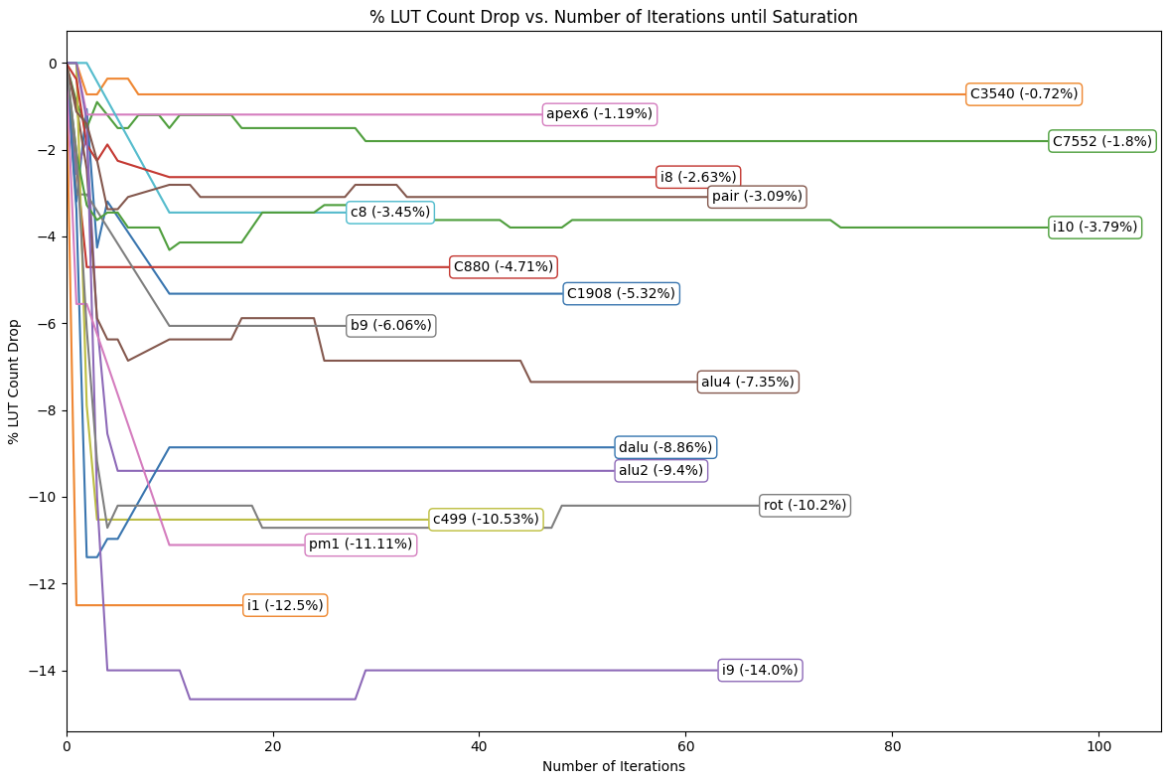
\includegraphics[width=\textwidth]{img/improvement.png}
        \caption{Marginal improvement versus iteration count. The labels mark the equality saturation point.}\label{fig:marginal:improvement}
    \end{subfigure}
    \hfill\vspace{4mm}
    \begin{subfigure}{0.47\textwidth}
        \centering
        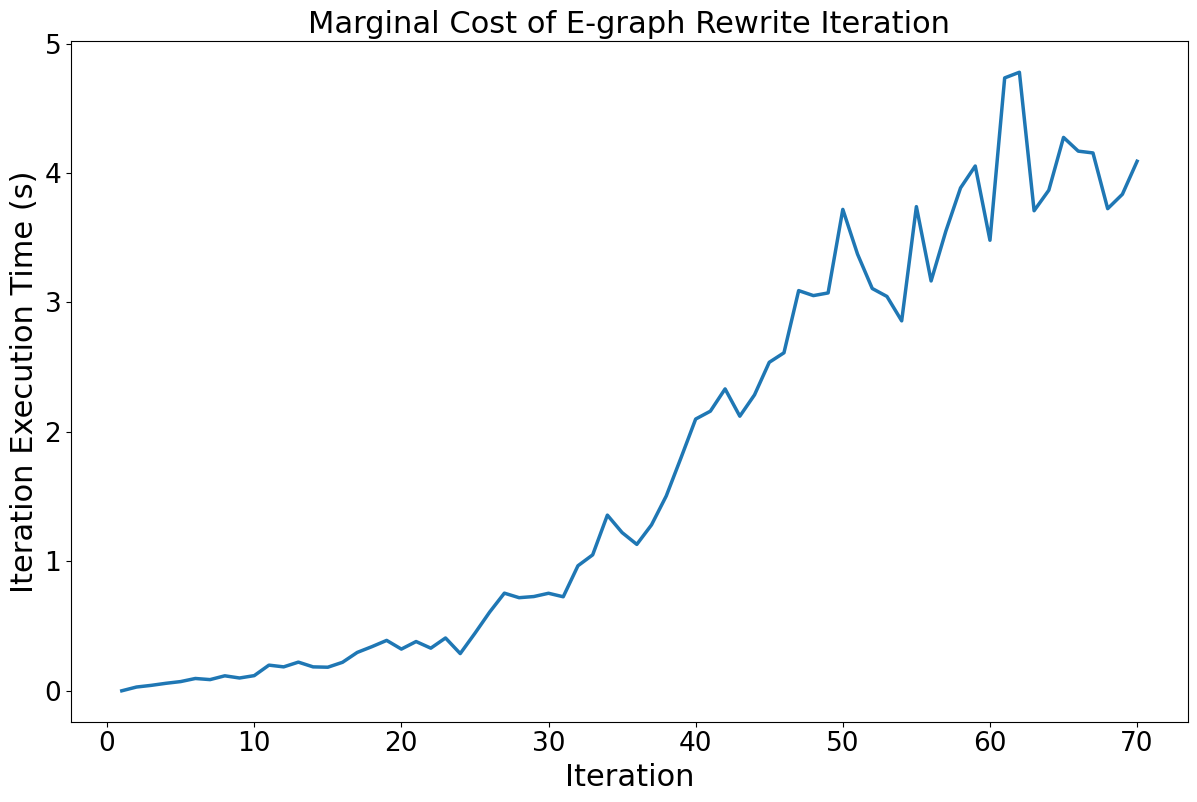
\includegraphics[width=\textwidth]{img/runtime_derivative.png}
        \caption{Marginal increase in runtime versus iteration count. Later iterations consume more time as the graph is larger.}\label{fig:marginal:runtime}
    \end{subfigure}
    \caption{Comparison of gains in QoR against e-graph size and runtime. Running a netlist to equality saturation requires more rewrite iterations, and hence a larger e-graph.}\label{fig:marginal}
\end{figure}

Given that \shortname{} is fundamentally a superoptimization tool, we want to
provide evidence that significant gains can be found within reasonable time
bounds. To that end, we empirically studied the marginal gains in QoR as
increasingly longer rewrite sequences are added to the e-graph. Within the
e-graph infrastructure, this phasing of applying rewrites and rebuilding the
union-find data structure is referred to as an \textit{iteration}. As shown in
Fig.~\ref{fig:marginal:improvement}, nearly all the performance gains are
discovered within the first 10 iterations---well before equality
saturation---suggesting that most of the optimizations are relatively local.
Some notable exceptions occur, such as `alu4' being reduced in size after the
40th iteration. Lastly, the growing runtime of e-graph exploration with each
iteration should be addressed. The marginal cost of executing an iteration of
rewrites becomes prohibitive as the e-graph becomes larger.
Fig.~\ref{fig:marginal:runtime} illustrates that after approximately the 30th
iteration, the marginal runtime rapidly increases into the 10s of seconds.

\subsection{Case Study: Pipelined Designs}\label{sec:results:retiming}
\begin{table*}[t]
    \centering
    \csvautobooktabular{data/mult.csv}
    \caption{LUT and flip-flop counts are report post-synthesis, but before placement and routing. CLB counts are reported after placement and routing.}\label{tab:multiply}
\end{table*}

Hardware designs with feed forward pipelines provide interesting opportunities
to apply register retiming and find a higher-level of area optimization. When
closing timing on FPGA designs, the critical path is often dominated by the
effects of routing congestion, more so than ASIC design. Hence, reducing the
cell count and circuit depth along the max delay path is a valid optimization
strategy for FPGA design. As a caveat, it is important to note that other work
has also observed the opposite trend~\cite{academicfpga}: decreasing depth too
much can strain the router. In any case, E-Pack can be utilized to reduce total
CLB usage. To elaborate, every CLB in the Ultrascale+ architecture contains 1
slice, which itself contains 8 LUTs and 16 flip-flops~\cite{ug574}.
Intuitively, a design that maps to CLBs efficiently will contain more
flip-flops than LUTs due to this 2:1 ratio. To test this hypothesis,
Table~\ref{tab:multiply} shows the results of a 32-bit pipelined multiplier
with a varying number of pipeline stages processed with E-Pack.

While the total drop is CLB usage is desirable, the area gains as a percentage
are modest due to the suboptimality of greedy e-graph extraction. Register
retiming rewrites vastly increase the design space. Unlike other logic
rewrites, register retiming changes the topology of the stateful
elements---i.e. the flip-flops. As a consequence, greedy extraction cannot take
into account the fanout of flip-flops. It can choose a poor design point with
less register fanout and a greater total number of registers. The few
regressions observed in mapping combinational logic
(Fig.~\ref{fig:marginal:improvement}) become more frequent and exacerbated in
sequential logic. While these results \textit{do} demonstrate that optimizing
for CLB count over raw cell count is a feasible strategy, a different
extraction method will be needed in future work.

\subsection{Case Study: Bit-Parallel Designs}\label{sec:results:scalability}
\begin{table}
    \centering
    \csvautobooktabular{data/alu.csv}
    \caption{Synthesis results of $n$-bit ALU}\label{tab:alu}
\end{table}

While the academic benchmarks enable direct comparisons to the rest of the
literature, the circuits are relatively small. On average, the designs map to
470 LUTs with \shortname{}. Among the \nimproved{} improved benchmarks in
Table~\ref{tab:results}, only three exceed 1000 LUTs. Although this e-graph
driven technology provides promising results for smaller benchmarks, FPGA
technology mapping is especially difficult---and important---for larger designs
with tens of thousands of LUTs. Through our case study on bit-parallel designs,
we demonstrate that \shortname{} performs just as well on large designs,
achieving area reductions without incurring excessive build times.

To test how \shortname{} scales with increasing numbers of LUTs, we created a
synthetic ALU benchmark and varied the input and output bit widths from 8 bits
to 4096 bits. Table~\ref{tab:alu} lists the LUT counts from the initial
synthesis by Vivado 2024, followed by the packed LUT counts. Even though the
1024-bit, 2048-bit, and 4096-bit ALU designs had up to 15,000 LUTs,
\shortname{} was able to achieve up to almost 15\% improvement over Vivado
within 5 minutes of extra build time. While longer runs lead to slightly better
improvements, these results demonstrate how \shortname{} can achieve area
reductions within a short period of time, even when input designs are scaled to
beyond 10,000 LUTs. In this specific case, \shortname{} can be used to audit
synthesis tools and perhaps even reverse-engineer adverse behavior. Hence,
\shortname{} proves to be a practical tool to run after a baseline synthesis by
Vivado or Yosys to quickly achieve better LUT packing with minimal time cost.

\section{Conclusion and Future Work}\label{sec:conclusion}
\todo{write the conclusion}

% Unstarted sections:
% [ ] Mult results: a big opportunity, but greedy extraction somewhat ruins it
% [ ] Future work

% Unstarted figures:
% [ ] A rewritten circuit (re-make by hand)

% MISC TODOS:
% (Matt): Explain the bumps and dips in the plot
% (Matt): Explain somewhere (prob results) that iterations/time *sometimes* mattter
% (Matt): Explain/mention rewrite figure in text

% use the ACM bibliography style
\bibliographystyle{IEEEtran}
\bibliography{IEEEabrv,references}

% \newpage
%%
%% If your work has an appendix, this is the place to put it.
% \appendix

\end{document}